\documentclass[a4paper]{article}
\usepackage{unifrrr}
\usepackage{graphicx}
\usepackage[latin1]{inputenc}
\usepackage{float}
\usepackage[colorlinks=false, pdfborder={0 0 0}]{hyperref}
\usepackage{verbatim}
\usepackage{hyperref}
\usepackage{cite}
\usepackage{bibgerm}
\usepackage[english]{babel}
\usepackage{listings}
\usepackage{color}
\definecolor{javared}{rgb}{0.6,0,0} % for strings
\definecolor{javagreen}{rgb}{0.25,0.5,0.35} % comments
\definecolor{javapurple}{rgb}{0.5,0,0.35} % keywords
\definecolor{javadocblue}{rgb}{0.25,0.35,0.75} % javadoc


\lstset{language=Java,
basicstyle=\ttfamily\footnotesize,
keywordstyle=\color{javapurple}\bfseries,
stringstyle=\color{javared},
commentstyle=\color{javagreen},
morecomment=[s][\color{javadocblue}]{/**}{*/},
numbers=left,
numberstyle=\tiny\color{black},
stepnumber=2,
numbersep=10pt,
tabsize=4,
showspaces=false,
showstringspaces=false,
captionpos=b}

\begingroup
    \catcode `\@ = 11
    \catcode `\~ = 13
    \catcode `\% = 12
    \protected\long\gdef\cmt@remove#1%~{\endgroup}
    \ifdefined~
        \global\let\cmt@old~
    \else
        \global\let\cmt@old\relax
    \fi
    \protected\gdef~{\begingroup\catcode`%=12
        \futurelet\next\cmt@}
    \protected\gdef\cmt@
      {\ifx%\next
           \expandafter\cmt@remove
       \else
           \endgroup\expandafter\cmt@old
       \fi}
\endgroup


\setcounter{secnumdepth}{4}
\setcounter{tocdepth}{4}

%--------------------------------------------------------------------


%The body of the LaTeX file
\begin{document}  



%Including of the title page. See titlepage.tex file
%Autor: Daniel Fasel daniel.fasel@unifr.ch
%Date: 10.01.2008
%Comment: An example of a title page file

%Starting the title page. A \begin command always ends with a \end command
\begin{titlepage} 
	%Center all the following stuff
	\begin{center}
		
		%Include the unifr.jpg file from ./images. \\ is a line break
		
\includegraphics[scale=2]{images/unifr.jpg}\\
		
		%Do a vertical space of 0.5 cm
		\vspace{0.5cm}
		
		
	
		\vspace{2cm}
		
		\begin{Large}
		Seminar Thesis: Applying Fuzzy Logic to Data Warehouses\\
		\end{Large}
		
		\vspace{2cm}
		
		%Start a huge font
		\begin{huge}
			%Sans serif
			{\sf \bf Fuzzy Concepts on Real Time Applications}
		\end{huge}
		
				
		\vspace{2cm}
		
		 %N\"uesch in capitals
		 Steve ASCHWANDEN \\
		 Stefan \textsc{N\"UESCH}\\
		
		\vspace{1.5cm}
		
		{\bf Examiner}\\
		Dr. Daniel Fasel\\
		\vspace{2.5cm}
		
		
		Wabern, \today\\
		
				
	\end{center}
\end{titlepage}


\pagenumbering{arabic}
\pagestyle{plain}
\newpage

\tableofcontents
\newpage

\section{Introduction}

The number of new tweets per second on the social media platform Twitter\footnote{https://www.twitter.com} is huge (over hundred thousand per second). To handle such a big amount of data, a scalable, fault-tolerant real-time framework has to be used. Storm was benchmarked at processing one million 100 byte messages per second per node (\cite{storm_site}). It allows to classify every new tweet, for example with a fuzzy logic approach. The so called ''Spout'' is responsible for fetching the tweets and the ''Bolts'' can do some transformation on the received data or persist them in some sort of storage. Cassandra\footnote{http://cassandra.apache.org} is an ideal solution for the given scenario, because it is a distributed, elastically scalable, highly available, fault-tolerant and column-oriented database.

\subsection{Problem Statement}

\subsubsection{Research Questions}\label{research_questions}
\vspace{0.5cm}
\begin{itemize}
\item How can fuzzy classifications be applied to Twitter feeds using Storm?
\item How can the results of such classifications be stored in a Cassandra column store?
\end{itemize}



\subsection{Objectives}

The main objective of this seminar project is to develop a simple prototype, which uses Storm to fuzzily classify messages from twitter feeds and store the results in a Cassandra NoSQL database.
The resulting application will use Storm on local system only (not on a cluster). Furthermore, only one fuzzy concept will be implemented in combination with a simple semantic analysis of the twitter feeds. However, the prototype shall be easily extensible with more complex analytics and further fuzzy concepts.


\subsection{Methodology}
This thesis will be conducted by prototyping. 
\subsection{Prototype}
The prototype resulting from this project will be a Java application based on the Storm library and using Cassandra for persistence. For analysing the twitter feeds, SentiWordNet will be used. 

\section{Existing Research}
\subsection{Twitter Trends}\label{twitter_trends}
There are several papers about twitter trends available. Some interesting approaches will be discussed in this chapter.\\

A few people from the Northwestern University implemented a topic classification algorithm for Twitter trends (\cite{leeEtAl2011}). To collect data for their experiments they used the information provided by the "What the trend"\footnote{http://whatthetrend.com/} website. They downloaded tweets which correspond to over 23'000 trending topics and randomly selected 768 topics to assign them to one of 18 selected topic classes like \textit{health, politics, technology} or \textit{movies}. They used supervised learning techniques to classify the trends to a topic class. The provided example (Figure \ref{techClass}) shows the hottest topics in the \textit{technology} class.
\begin{figure}[h!]
	\centering
	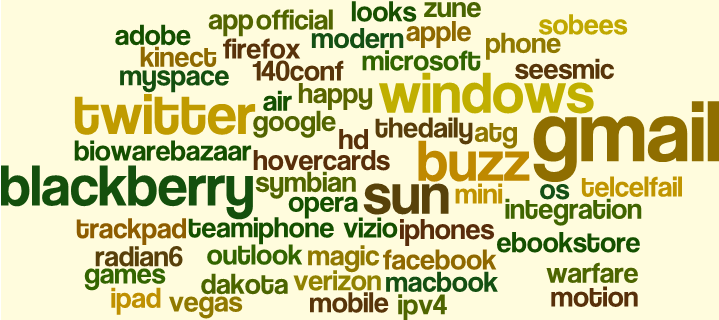
\includegraphics[scale=0.35]{images/technologyClass.png}
	\caption{Technology class topics \cite{leeEtAl2011}}
	\label{techClass}
\end{figure}

Another paper has the focus on the trend detection (\cite{Mathioudakis2010}). Two guys from the computer science department at the University of Toronto developed a monitor (Figure \ref{monitorArchitecture}) for Twitter trends in real-time. They split their implementation into a front and back-end part. The \textit{TwitterListener} separates the tweet information into fields (tweet text, author, timestamp) and exports two feeds. Text and timestamp go to the \textit{Bursty Keywords Detection} module. This module computes a set of bursty keywords for every tweet and tries to find other tweets in the past which were assigned to the same set (\textit{Bursty Keywords Grouping}). If the system has found enough tweets it will create a new trend with the corresponding description (\textit{Trend Analysis}). The \textit{Lucene}\footnote{http://lucene.apache.org/core/} module needs all the fields from the tweet. Apache Lucene is responsible for indexing the tweets. This is important to get feeds from the past, because the Twitter API had some restrictions for requests that date further back in time. The \textit{Interface} module will present the trends on a webpage.
\begin{figure}[h!]
	\centering
	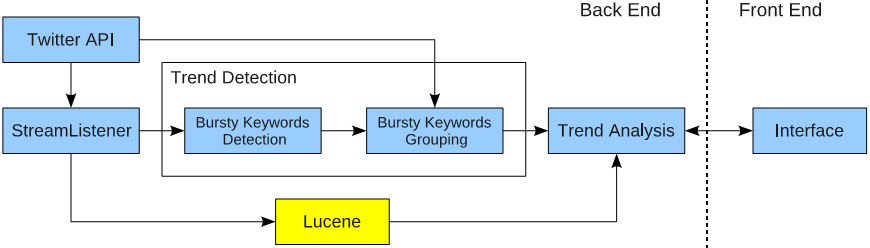
\includegraphics[scale=0.45]{images/monitorArchitecture.png}
	\caption{Architecture of the Twitter Monitor \cite{Mathioudakis2010}}
	\label{monitorArchitecture}
\end{figure}

\subsection{Sentiment Analysis}\label{section_sentiment}
The sentiment analysis of a tweet is also a well-covered topic by the computer science community.\\ 

Members of the University of Edinburgh wrote a paper with the title: "Twitter Sentiment Analysis: The Good, the Bad and the OMG!" (\cite{KouloumpisWM11}). They took tweets and did some preprocessing steps first. Replace abbreviations by their actual meaning (e.g. 'BRB' goes to 'be right back') and repeated characters are replaced by single characters (e.g. 'happyyyy' goes to 'happy'). Finally, each word was assigned to a POS-tag (Part-of-Speech). After that, a number of feature values was calculated. The \textit{n}-gram feature which is a contiguous sequence of \textit{n} items from a given tweet. The Part-of-Speech feature count the number of verbs, adverbs, adjectives, nouns and any others. The MPQA subjectivity lexicon\footnote{http://mpqa.cs.pitt.edu/lexicons/subj\_lexicon/} (similar to SentiWordNet) was used to calculate a positive, negative and neutral value based on the presence of any words from the lexicon. Emoticons and abbreviations - Micro-blogging feature - define a feature too (by the use of the Internet Lingo Dictionary and various internet slang dictionaries). To train an AdaBost model they used over 20'000 tweets. The usage of the Part-of-Speech feature didn't improve the performance of the classifier. The micro-blogging feature was clearly the most useful. With the best combination of the features they get an average accuracy of 0.75 on different test sets (Figure \ref{sentimentAccuracy}).
\begin{figure}[h!]
	\centering
	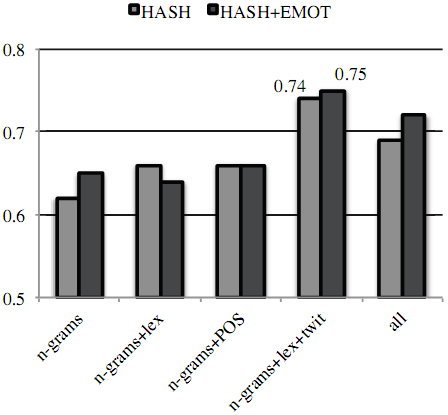
\includegraphics[scale=0.5]{images/sentimentAccuracy.png}
	\caption{Average accuracy with different features \cite{KouloumpisWM11}}
	\label{sentimentAccuracy}
\end{figure}

\subsection{SentiWordNet}\label{sentiWordNet}
SentiNetWord\footnote{http://sentiwordnet.isti.cnr.it/} is an English dictionary for opinion mining (OM, also known as sentiment classification). The goal was to decide for every word of the WordNet\footnote{http://wordnet.princeton.edu/} if it has a positive, negative or neutral meaning. WordNet is a large lexical database of nouns, verbs, adjectives and adverbs provided by the Princeton University. The developers calculated for every word three values between 0.0 and 1.0 and they had to sum up to one. They labelled different entries of the dictionary manually to define a ground truth for the training set. Then a set of classifiers was trained with the provided data. After these steps the classifiers were able to calculate the corresponding values of the remaining words which weren't in the training data samples. Since the first version of SentiWordNet in 2006 a lot of improvements are done, the actual version is 3.0.0. It's freely available for research approaches.\\
The dictionary consists of 117'659 entries (69.8\% nouns, 15.4\% adjectives, 11.7\% verbs and 3.1\% adverbs). If we take a closer look at the calculated values (in SentiNetWord 1.0.0) we can see that most of the words are objective (about eighty percent are greater than 0.75). Only a few words are positive (0.48\% \textgreater \ 0.75; about 560 words) or negative (1.28\% \textgreater \ 0.75; about 1500 words).\\
The resulting dictionary can be downloaded on the research website of SentiWordNet and has the following columns (tab separated):
\begin{enumerate}
	\item Part of speech (noun, verb, adjective, adverb)
  \item ID
	\item Positive score
	\item Negative score
	\item The words (plural because of synonyms)
	\item Glossary (the word in a given context)
\end{enumerate}
The neutral (objective) score of the word can be calculated by 1 - (Positive score + Negative score).

\section{Technologies}

\subsection{Storm}
Storm is an open source distributed real-time computation system and programming language independent with the following nice properties:
\begin{itemize}
	\item \textbf{Easy to program} An implementation of a real-time processing tool from scratch needs a lot of time and effort. With Storm, a simple working topology can be created within a few hours 
	\item \textbf{Programming language independent} The easiest way is to develop in a JVM-based language, but Storm supports any language if you use or implement a small intermediate library 
	\item \textbf{Fault-tolerant} If a \textit{worker} is going down, the cluster will reassign tasks when necessary 
	\item \textbf{Scalable} Add or remove machines to the cluster. Storm will reassign tasks to new machines as they are available or distribute the tasks from the removed machines to the others which are still there 
	\item \textbf{Reliable} Storm guarantees that every message will processed at least once. If an error occurs, the messages can be processed more then once. But a message will never be lost 
	\item \textbf{Fast} Storm can process one million 100 byte per second per node on a machine with two processors (Intel E5645@2.4Ghz) and a 24 GB memory 
\end{itemize}
\subsubsection{Components}\label{storm_components}
A Storm \textit{topology} consists of two main components:
\begin{itemize}
	\item \textit{Spouts} are responsible to fetch the data from a source (e.g. text file, Twitter streaming API)
	\item \textit{Bolts} are responsible for the transformations of the fetched data
\end{itemize}
The spout acts as the source of the data flow and the last bolt is the sink which store the output to a database. The output of one component goes always to the input of the next, therefore no data will flow through an already visited node. A simple example should help to illustrate the components of the Storm architecture (Figure \ref{storm_example}):\\

\begin{figure}[h!]
	\centering
	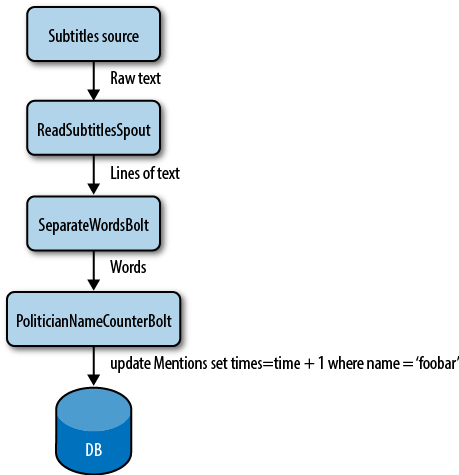
\includegraphics[scale=0.5]{images/storm_example.png}
	\caption{Storm example \cite{leibiusky2012}}
	\label{storm_example}
\end{figure}
All the spoken words during the TV news show will be stored in a text file. If a new sentence was written into the file the spout hands them to the responsible bolt which separate the sentence into words. This stream of words is passed to another bolt that compares each word to a list of politician's names. If there is a match, the second bolt increases the counter for that name in a storage. To check the number of occurrence, query the database which is updated in real-time.\\
Typical uses cases for a Storm application can be:
\begin{itemize}
	\item \textbf{Processing streams} This is the case in the shown example 
	\item \textbf{Continuous computation} Continuously send data to the clients so they can update and display results in real-time, for example as site metrics 
	\item \textbf{Distributed remote procedure call} Easily parallelize CPU-intensive operations
\end{itemize}
\subsubsection{Grouping}
After the implementation of the spouts and bolts for the topology, they have to be connected with each other. Stream grouping defines which stream are consumed by each bolt and how they will be consumed. Strom provides different grouping types: 
\begin{itemize}
	\item \textbf{Shuffle} The most commonly used grouping. It sends each tuple emitted by the source to a randomly chosen bolt. If there are no dependencies between the emitted tuples (e.g. fuzzy classification of a tweet) this grouping method is used 
	\item \textbf{Fields} Control how the tuples will be distributed, based on the emitted fields. It guarantees that a set of values for the same combination of fields will be sent to the same bolt. This is useful to implement a MapReduce functionality 
	\item \textbf{All} Sends a single copy of each tuple to every receiving bolt (e.g. resetting a counter, refreshing a cache) 
	\item \textbf{Custom} Create a custom stream grouping by implementing the\\
\textit{back.type.storm.grouping.CustomStreamGrouping} interface 
\end{itemize}
\subsubsection{Technical Details}
In a Storm cluster there are 2 node types, a \textit{master} node and \textit{worker} nodes. The master node runs a daemon called '\textit{Nimbus}', which is responsible for code distribution, task assignment and failure monitoring. A portion of the topology is running on the worker nodes (responsible daemon is called 'Supervisor'). A topology runs across multiple worker nodes on different machines. Since Storm keeps the states of the cluster either in '\textit{Zookeeper}' or on local disk, the daemons are stateless and can fail or restart without disturbing the system.\\
Storm uses an advanced, embeddable networking library called zeromq (0mq, http://zeromq.org/), which provides features that make Storm possible. Some characteristics of zeromq:
\begin{itemize}
	\item Act as a concurrency framework
	\item Faster than TCP, ideal for clustered products and supercomputers
	\item Carries messages across in-process, IPC (inter-process communication), TCP and multicast
	\item Asynchronous I/O model for scalable multi-core applications
	\item Connect sockets N-to-N 
\end{itemize}
Storm topologies can run in two different modes. The \textit{local} mode is a single Java Virtual Machine on a local machine. This mode is used for developing, testing and debugging. The other possibility is to run the software on different \textit{remote} machines. But there are no debugging information in the production mode.\\

The difference between a traditional BigData approach like Hadoop\footnote{http://hadoop.apache.org/} and Storm is the paradigm that it addresses. Hadoop fundamentally a batch processing system. The results are available after the whole data was distributed over the whole system. The construction of topologies that transform unterminated streams of data is supported by Storm. A Storm topology will never stop running (until termination by user), Hadoop jobs will stop after all available data (at starting time) proceeded by the system.

\subsection{Cassandra}
Eben Hewitt \cite{hewitt2010cassandra} explained Cassandra with only 50 words:\\

"Apache Cassandra is an open source, distributed, decentralized, elastically scalable, highly  available, fault-tolerant, tuneably consistent, column-oriented database that bases its distribution design on Amazon's Dynamo and its data model on Google's Bigtable. Created at Facebook, it is now used at some of the most popular sites on the Web."\\

The data store is an open source Apache project available at http://cassandra.apache.org. Cassandra originated at Facebook in 2007. It should solve the company's inbox search problem, because they had to deal with large volumes of data. The project was moved to Apache in March 2009.

\subsubsection{Properties}
Cassandra has some interesting properties:

\paragraph{Elastic Scalability }
There are two different types of scaling. Add more hardware capacity and memory to the existing way is one way to handle a greater number of requests. This approach is called vertical scaling. Horizontal scaling will add more machines to distributed the incoming data over multiple nodes. This will decrease the amount of data for every machine. Elastic scalability is a specialization of the horizontal scaling where the cluster can scale up and scale back down, depending on the current load. Cassandra is able to handle new machines on-the-fly without the need for restarting the process or manually rebalancing of the data. 
\paragraph{High Availability and Fault Tolerance}
Machines in the cluster will have technical issues from time to time. Cassandra is able to handle replaced failed nodes without downtime. Also, replication of data to multiple data center is possible to prevent downtime if a data center experiences a catastrophe like a fire. 
\paragraph{Tuneable Consistency}
Consistency means that a read operation returns the last written value from the database. But a database system cannot implement all three components of the CAP theorem\cite{Gilbert:2002:BCF:564585.564601} and the focus of Cassandra are Availability and Partition tolerance (AP). Therefore, the consistency is not guaranteed. But it allows to configure the degree of the consistency in balance with the level of availability: 
\begin{itemize}
	\item \textbf{Strict consistency} Also called sequential consistency. It's the highest level of consistency and it requires that a read will always return the recently written value in the database. If you have only a single machine with one processor (and one processor clock) the last written value is easy to find. But if there are geographically dispersed data centers, it becomes much more slippery. A global clock which can timestamp all operations, regardless of the data location or how many services are needed to determine the response, is required 
	\item \textbf{Causal consistency} A weaker form of the strict approach. It uses a much more semantic approach and it does away with the fantasy of a single clock which can be synchronized without creating a bottleneck. The idea is that writes which are potentially related must be read in sequence. Writes are inferred not to be causally related, if two operations suddenly write to the same filed (operations must be different and unrelated). But if there is enough time between two write operations, we assume that they are causally related. Therefore, causal consistency says that causal writes must be read in sequence 
	\item \textbf{Weak (eventual) consistency} All updates will propagate throughout all of the machines in a distributed system. Of course, this will take some time. But It could be possible that all replicas will be consistent 
\end{itemize}
The user of Cassandra can control the number of replicas to block on for all updates (Tunable consistency). This can be done by setting the \textit{level of consistency} against the \textit{replication factor}. With the replication factor the client can define the level of consistency, but a higher level implies a lower performance of the system. The factor controls the number of nodes in the cluster where you want to distribute the updates (add, update and delete). The number of replicas which have to acknowledge a write operation or respond to a read operation to declare this operation as successful is defined by the consistency level.

\paragraph{Raw-Oriented}
Cassandra is a column-oriented database, it represents their data structures in sparse, multidimensional hashtables. For every given row you can have many columns, but they doesn't have to be the all the same like in the relational model. A unique key makes the data accessible. One advantage of Cassandra is that you don't have to define what the data structure must look like or what fields you will need. This implies also that you can add or remove new fields on-the-fly without disturbing the system. This is ideal if you use an agile development methodology and you don't have time to define the entire database schema at the beginning of the project.

\paragraph{Schema-Free}
The first step to define a Cassandra database is the creation of a \textit{keyspace} which is a logical namespace to hold \textit{column families} and some configuration properties (e.g. replication factor). The column families are names for associated data and a sort order. Because the tables are sparse, the data can just be added using arbitrary columns. There is no need for modeling data up front using data modeling tools and then creating queries with complex join statements. With Cassandra, the user can first create the queries and the system will provide the data around them.

\paragraph{High Performance}
Cassandra was designed to take full advantage of multiprocessor/multicore machines and run on multiple of these machines in data centers. It should be scale to hundreds of terabytes and stay consistent. People from the University of Toronto analysed the performance of Cassandra \cite{rabEtAl2012}. They defined some different workloads to create scenarios. One was with 50\% inserts, 25\% reads and 25\% scans. Two independent clusters are used where each has about 16 Linux nodes (Intel Xeon quad core CPU's, 16GB of RAM, 148GB disk space). The nodes are connected with a gigabit Ethernet network over a single switch. The strength of Cassandra is clearly visible (Figure \ref{throughput_cassandra}), because the throughput with only one node is lower than other ones. If the number of nodes was increased, the gap between Cassandra and all the other tested systems is significant.

\begin{figure}[h!]
	\centering
	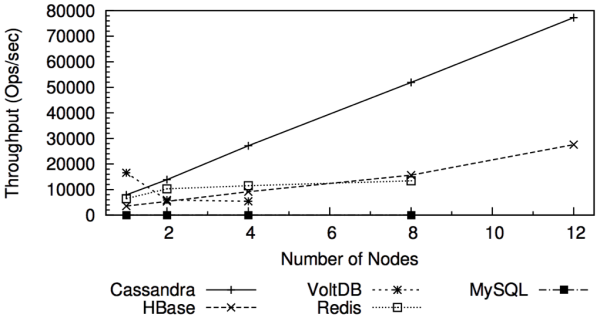
\includegraphics[scale=0.5]{images/throughputCassandra.png}
	\caption{Performance of different distributed database systems \cite{rabEtAl2012}}
	\label{throughput_cassandra}
\end{figure}

The authors of the paper concluded their paper with the following words:\\

"In terms of scalability, there is a clear winner throughout our experiments. Cassandra achieves the highest throughput for the maximum number of nodes in all experiments with a linear increasing throughput from 1 to 12 nodes."

\subsubsection{Data model}
Cassandra using the data model from the BigTable approach from Google \cite{chang2008bigtable}. To illustrate the components of this model we take a look at an example application. Assume the user want to store a large collection of webpages and some further information. BigTable is a persistent, multidimensional sorted map and the map is indexed by a \textit{row} key, \textit{column} key and a \textit{timestamp}. For the webpage collection the URLs are the row keys, various aspects of the webpages are column names. Assume the CNN site want to be stored (Figure \ref{model_bigtable}).
\begin{figure}[h!]
	\centering
	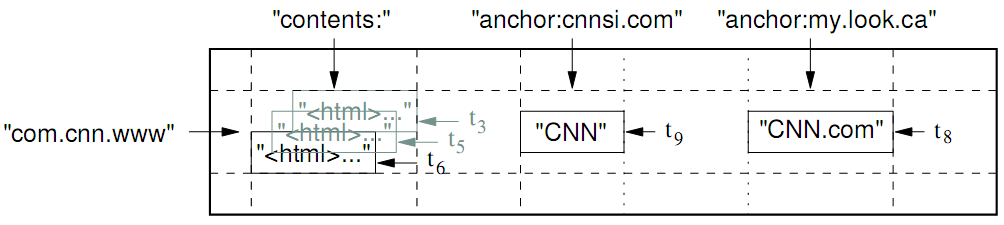
\includegraphics[scale=0.4]{images/modelBigTable.png}
	\caption{Illustration of the BigTable data model \cite{chang2008bigtable}}
	\label{model_bigtable}
\end{figure}
The row name is the reversed URL. The map is sorted by the row key and we want to group the domains together with their corresponding subdomains (e.g. com.cnn.sport). The whole content of the page (source code) is kept in the contents column family. There are three different versions at timestamp t$_{3}$, t$_{5}$ and t$_{6}$ because the content of the page changes over time. Each cell can contain multiple versions of the data, indexed by 64-bit integers timestamps. The anchor column family contains the name of the anchors that reference the CNN page. The Sports Illustrated (column name is \textit{anchor:cnnsi.com}) and the MY-look (\textit{anchor:my.look.ca}) pages have a link to CNN. The column name contains information too, that is not possible with a relational database model. Every column key is named using the syntax: \textit{family:qualifier}. A column family has to be created before data can be stored under any column key in that family.


\section{Implementation}\label{implementation}
The following chapter describes the prototype developed by the authors to answer the question raised in chapter~\ref{research_questions}. Firstly, several central parts of the prototype are described in detail. Thereafter, the chapter~\ref{section_topology} shows how these parts are connected within the application. Finally, the chapter~\ref{section_api} describes how the prototype can be extended with new functionality.


\subsection{Data Collection}
To access Twitter data, a simple Storm Spout (cf. \ref{storm_components}) is used. At the initialization of this component, an \textit{oAuth} connection to Twitter is created. The oAuth authentication framework will not be discussed in this report, however, further details can be found at \url{http://oauth.net}. After initialization, the spout simply processes each tuple by assigning it a unique identifier (\texttt{UUID}) and forwarding it into the prototype topology (cf. chapter~\ref{section_topology}).

\subsection{Classification}
As stated in chapter \ref{research_questions}, the goal of the implementation is to enable fuzzy classification of tweets. To achieve fuzzy classification, two steps are necessary. First, there has to be a mapping of numerical values to the tweets. This step will e referred to as discrete classification in the following. Second, a fuzzy membership function must be applied to this discrete classification. This step is called fuzzy classification. This chapter details the implementation of these steps in the presented prototype.\\

\subsubsection{Discrete Classification}\label{section_discrete}
\begin{figure}[h!]
	\centering
	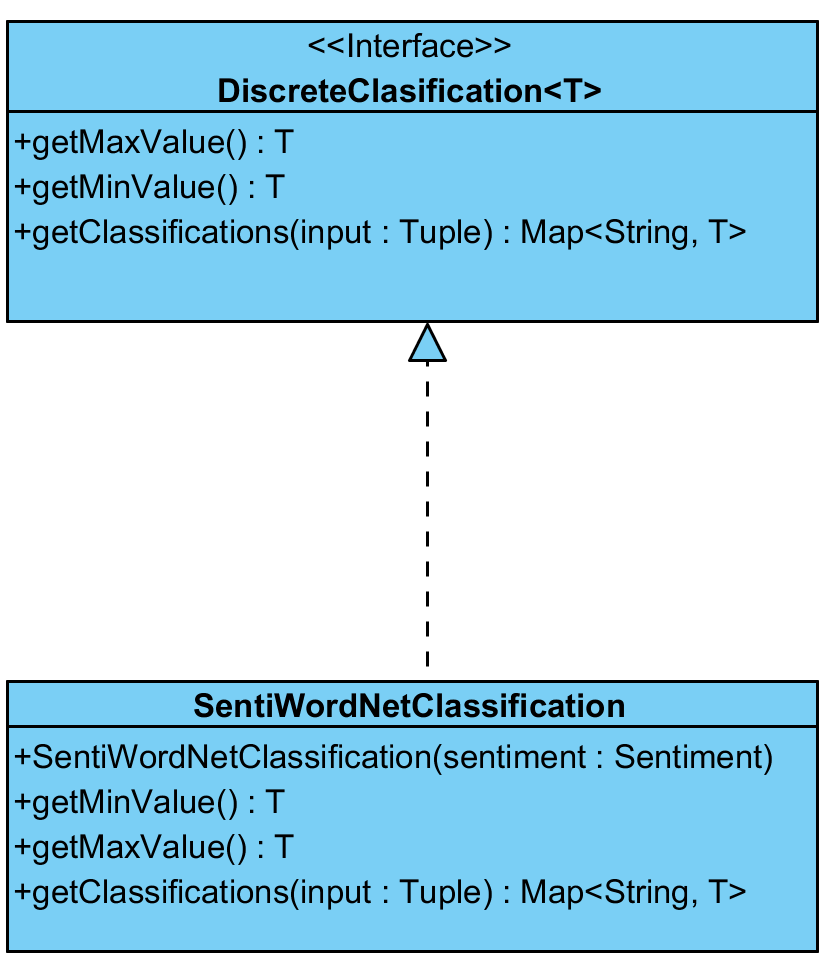
\includegraphics{images/uml_discrete.png}
	\caption{Discrete Classification - Interface and Sample Implementation}
	\label{uml_discrete}
\end{figure}
To enable discrete classification, the prototype provides an interface \texttt{DiscreteClassification<T>}. The interface is generically typed with type T, which needs to be an extension of the Java Number class (\texttt{java.lang.Number}). This generic typing provides the possibility to map different types of numerical values to tweets, such as integers or floating point numbers. An implementation of the interface specifies the numerical type according to the mapping or calculation it performs.\\
In order to achieve numerical classification of tweets, an implementation needs to specify a range of possible values, as well as the actual calculation of these values. Accordingly, the interface provides the following methods (as depicted in figure~\ref{uml_discrete}):
\begin{itemize}
\item \texttt{getMinValue()}: This method returns the minimum value of the classification range.
\item \texttt{getMaxValue()}: This method returns the maximum value of the classification range.
\item \texttt{getClassifications()}: The actual calculation of the numerical values. As input, the method receives the tweet in form of a \texttt{Tuple}, which is a wrapper class used by Storm. Currently, the interface is designed as to support word-by-word classification of the tweets, therefore it returns a map which relates the word (map key) to the calculated numerical value (map value).
\end{itemize}

\subsubsection{Sample Implementation}
To be able to answer the questions stated in \ref{research_questions}, sample implementations for both discrete and fuzzy classification need to be provided by the prototype. The authors chose to use SentiWordNet, explained in chapter~\ref{sentiWordNet}, to discretely classify the tweets. More specifically, the class \texttt{SentiWordNetClassification} may be initialized to either rate the negative or the positive sentiments expressed in a tweet. As a word in the SentiWordNet database may have both a positive and a negative rating, and as these ratings are not necessarily correlated, the positive positive and the negative ratings are treated as different classifications. To calculate both positive and negative sentiments for tweets, two separate bolts (cf. chapter~\ref{section_topology}) could be added to the prototype topology.\\

\lstset{language=Java,caption={SentiWordNet Dictionary Creation},label=sentiwordnet_dict}
\begin{lstlisting}
Map<String, Double> dict = new HashMap<>();
InputStream is = this.getClass().getClassLoader().getResourceAsStream(SWN_PATH);
BufferedReader csv =  new BufferedReader(new InputStreamReader(is));
String line = "";
while((line = csv.readLine()) != null){
	// The file is tab separated
	String[] data = line.split("\t");
	// Get entry word
	String[] words = data[WORD_POSITION].split(" ");
	// There can be multiple words
	for(String w : words)
	{
		// Remove the '#'-sign from the words
		String[] w_n = w.split("#");
		if(!dict.containsKey(w_n[0])){
			// implementing class has to supply correct position
			dict.put(w_n[0], Double.parseDouble(data[position]));
		}
	}
}
csv.close();
return dict;
\end{lstlisting}

Listing~\ref{sentiwordnet_dict} shows the java code for creating the SentiWordNet dictionary. As visible from the code between line 6 to line 15, each word is added to the dictionary only once. Furthermore, all special characters are removed, and any context information is ignored. This approach does not consider several features of the original SentiWordNet dictionary, such as the word class (adjective, nouns, adverbs, etc.) and combinations of words (e.g. certain idioms), among others. While such information may be beneficiary for the precision of the word ratings, the described approach allows for a simple calculation of roughly adequate ratings. \\
The dictionary created by the code shown in listing~\ref{sentiwordnet_dict} is the central part of word-by-word classification. The tweets supplied to the \texttt{getClassifications()} method will be split into words. Thereafter, the positive or negative value for each word is looked up in the dictionary, if any exists.




\subsubsection{Fuzzy Classification}\label{fuzzy_classification}
\begin{figure}[h]
	\centering
	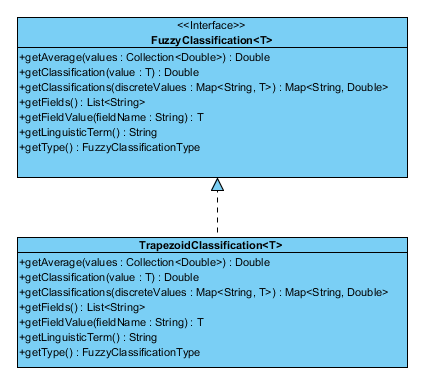
\includegraphics{images/uml_fuzzy.png}
	\caption{Fuzzy Classification - Interface and Sample Implementation}
	\label{uml_fuzzy}
\end{figure}

Similar to the discrete classification (cf. chapter~\ref{section_discrete}), the prototype provides an interface for defining fuzzy classifications. This interface also features the same generic numerical type. In contrast to the discrete classification, however, the generic typing refers to the type of input which is used to calculate to fuzzy classification. The output is defined as a normalized \texttt{double} value, that is to say a value between 0 and 1.\\
The interfaces provides a caller with the following methods, as shown in figure~\ref{uml_fuzzy}.
\begin{itemize}
\item \texttt{getAverage()} This convenience method calculates the average of all classification values supplied as input. It expects these values to be already fuzzily classified.
\item \texttt{getClassification()} Returns the fuzzy classification for a single discrete value.
\item \texttt{getClassifications()} For each value of the input map, this method calls \texttt{getClassification()}, and adds it to the output map which is finally returned. In both maps, the keys are the words of a tweet to which a numerical value is mapped.
\item \texttt{getFields()} Used to support the Storm data flow architecture (cf. chapter~\ref{TODO}), this method returns a list of fields which define the fuzzy classification. Generally, these are the initialization parameters for this classification, as shown in the subsequently described sample implementation.
\item \texttt{getFieldValue()} Returns the value of a field declared by \texttt{getFields()}. Again, this method is used for support of Storm.
\item \texttt{getLinguisticTerm()} Returns the linguistic term associated with this fuzzy classification.
\item \texttt{getType()} The \texttt{FuzzyClassificationType} returned by this method is used when storing the classification, as detailed in chapter~\ref{section_api}.
\end{itemize}

\subsubsection{Sample Implementation}
\begin{figure}[h]
	\centering
	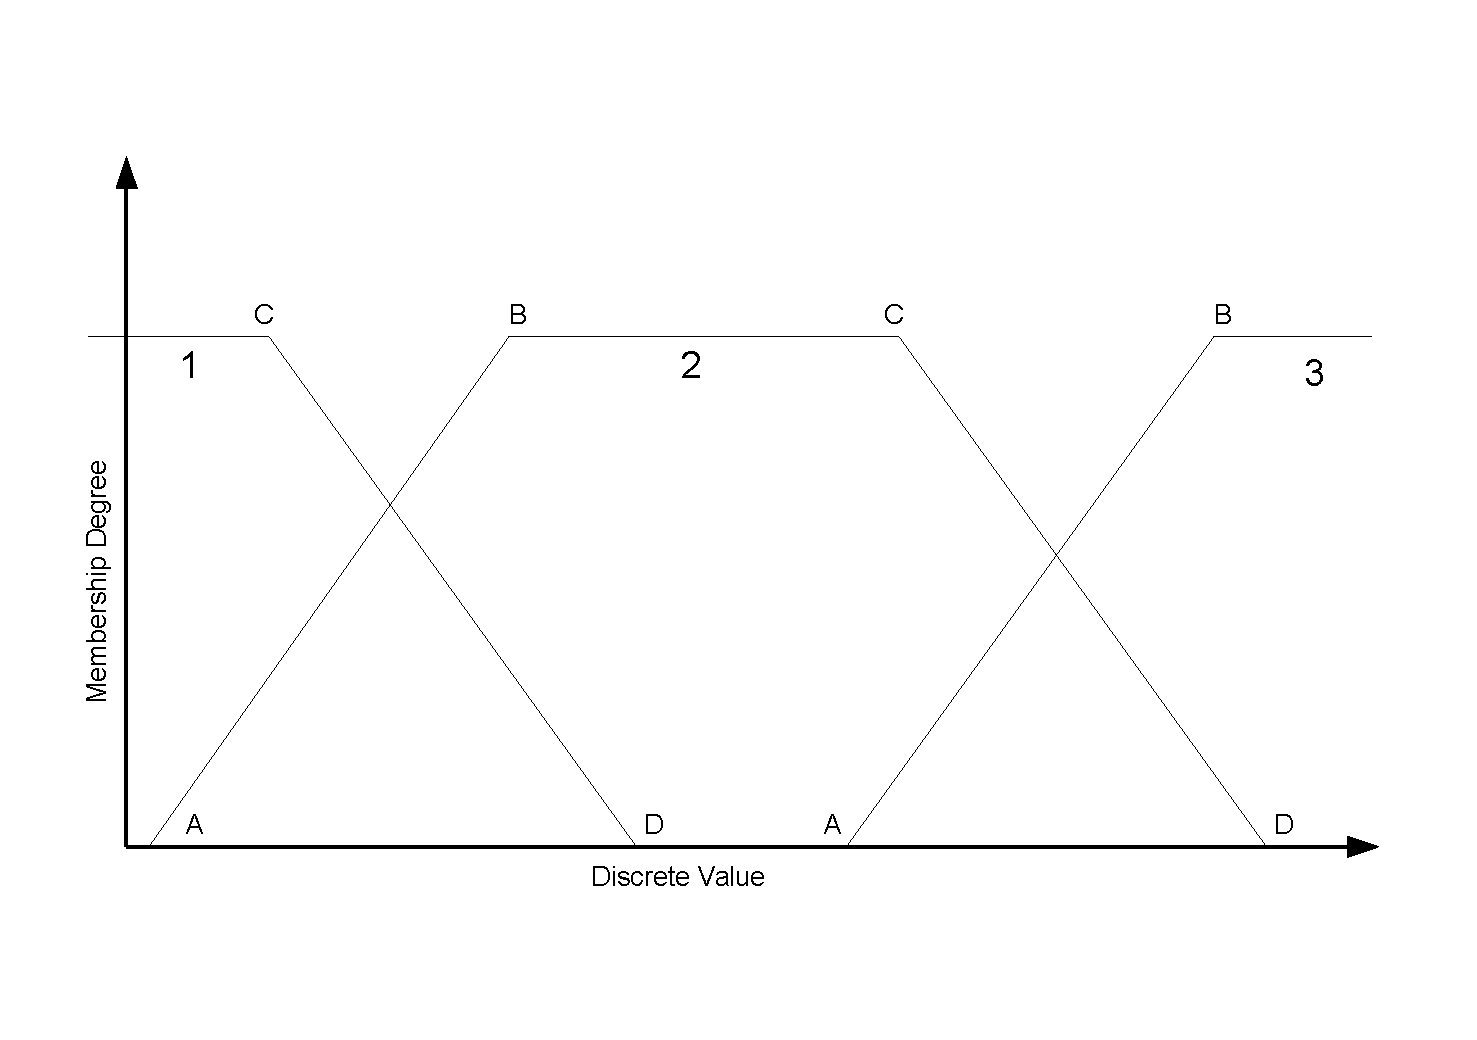
\includegraphics[scale=0.5]{images/trapezoid.pdf}
	\caption{Trapezoid Member ship function (based on \cite{faseld2012}, p. 74)}
	\label{trapezoid_functions}
\end{figure}

For the sample implementation of a fuzzy classification, a trapezoid membership function was chosen. Examples of trapezoid function are depicted in figure~\ref{trapezoid_functions}, as adapted from \cite{faseld2012}, p. 74. There are four distinct boundaries which define such a function, namely the \textit{lower limit} (labelled with A), the \textit{lower support limit} (B), the \textit{upper support limit} (C) and the \textit{upper limit} (D). Furthermore, the implementation considers three types of trapezoid functions. Label 1 shows a \textit{left open} function, meaning that all discrete values below the upper support limit will be classified with a membership degree of 1. Label 2 shows a \textit{closed} function, and label 3 a \textit{right open} function.\\
To reflect these properties, the concrete implementation of the \texttt{FuzzyClassification} interface in the prototype is initialized with five parameters. The first parameter is used to define the linguistic term, while the four subsequent parameters define the lower limit, the lower support limit, the upper support limit and the upper limit respectively. To define left open function, the class is initialized with lower limit and lower support limit set to \texttt{null}, and vice versa for right open functions.\\

The calculation of the actual fuzzy value for a discrete value is done as shown in listing~\ref{fuzzy_calc}. The method \texttt{isOne()} will return true if a value is between the lower and the upper support limit. \texttt{isRising()} will return true if the value is between the lower limit and the lower support limit, and vice versa for \texttt{isFalling()}. This distinction is necessary to calculate the correct membership degree of the discrete value, which is done by normalizing the difference between the lower support limit and the lower limit (in case of \texttt{isRising() == true}) or between the upper support limit and the upper limit (in case of \texttt{isFalling() == true}), as shown in listing~\ref{get_difference}
\lstset{language=Java,caption={Calculation of Fuzzy Values},label=fuzzy_calc}
\begin{lstlisting}
if (this.isOne(value)) {
	return 1.0;
} else if (this.isRising(value)) {
	return this.getDifference(this.lowerLimit, this.lowerSupportLimit, value, false);
} else if (this.isFalling(value)) {
	return this.getDifference(this.upperSupportLimit, this.upperLimit, value, true);
} else {
	return 0.0;
}
\end{lstlisting}
\lstset{language=Java,caption={Membership degree calculation},label=get_difference}
\begin{lstlisting}
double diff = highValue.doubleValue() - lowValue.doubleValue();
double relValue = value.doubleValue() - lowValue.doubleValue();
return isFalling ? 1.0 - (relValue / diff) : relValue / diff;
 
\end{lstlisting}

Finally, for the usage with Storm as described in chapter~\ref{TODO_storm}, the \texttt{getFields()} method will return the names of the fields defining the four limit parameters. These values are later retrieved to persist together with the fuzzily classified values.

\subsection{Persistence}
The persistence of tweets and the associated fuzzy classification is implemented in a rather simple way. A \texttt{CassandraBolt} receives tuples from the topology (cf. chapter~\ref{section_topology}). For each tuple, it calls the \texttt{CassandraConnector}, which uses a simple \texttt{INSERT} statement to write the values to the connected Cassandra database.

\subsection{Topology}\label{section_topology}
\begin{figure}[h!]
	\centering
	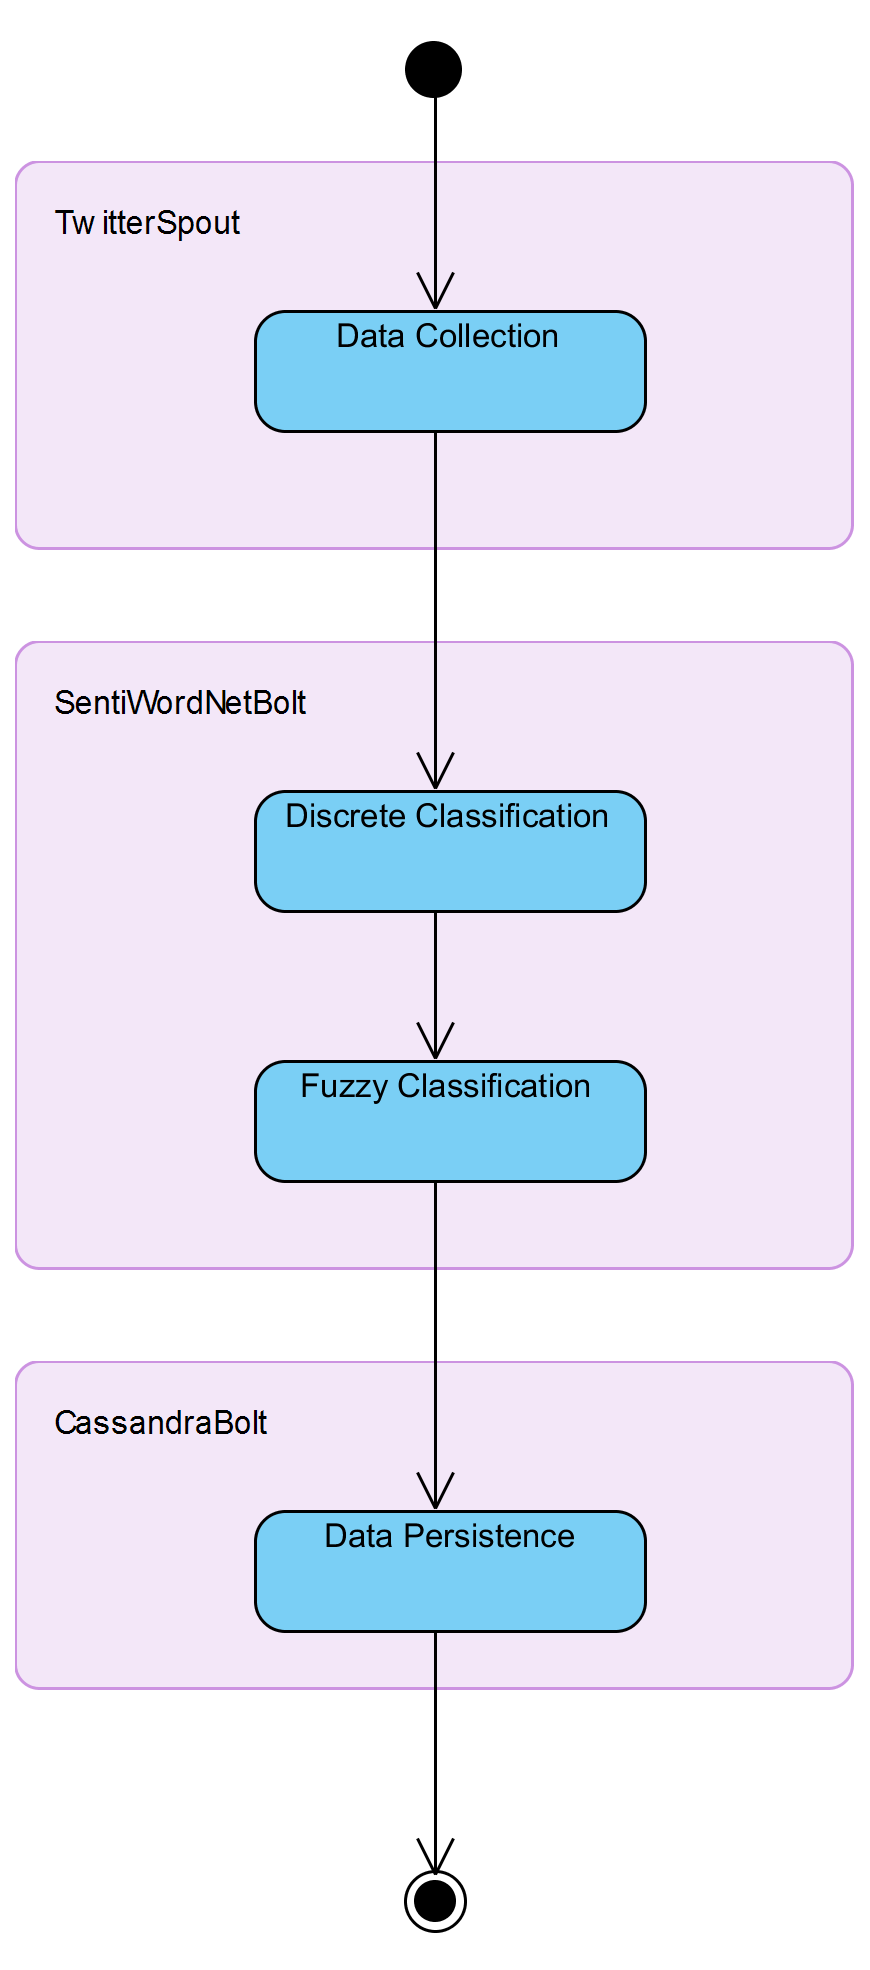
\includegraphics[scale=0.8]{images/state.png}
	\caption{State Chart for Tuple Processing}
	\label{uml_states}
\end{figure}
In the previous chapters, the central part of the prototype have been laid out in detail. The connection of these parts into a running system is best illustrated using the following small source code sample. The listing shows the creation of Spout and Bolts in the \texttt{MainTopology} class as well as their registration with a \texttt{TopologyBuilder}. In addition, figure~\ref{uml_states} depicts the life cycle of tweets collected and analysed by the topology.

\lstset{caption={Topology Setup},label=topology_setup}
\begin{lstlisting}
builder.setSpout("twitterStream", new TwitterSpout(oauth_consumer_key, oauth_token,
	oauth_consumer_secret, oauth_access_token_secret, track));

SentiWordNetBolt<Double> bolt = SentiWordNetFactory.createPositiveSentiWordNetBolt();
builder.setBolt("swnPositiveBolt", bolt).shuffleGrouping("twitterStream");
builder.setBolt("cassandraBolt", new CassandraBolt(), 1).shuffleGrouping("swnPositiveBolt");
\end{lstlisting}	

The first line shows the creation of the \texttt{TwitterSpout}. It retrieves tweets from Twitter, and emits them as tuples into the Storm framework.\\
The next lines show the creation and the registration of the Bolts used in the prototype. Firstly, a Bolt for positive classification is instantiated by a call to the \texttt{SentiWordNetFactory} and registered with the topology. When a tuple is emitted from the \texttt{TwitterSpout}, it will be sent to this Bolt. Upon arrival, the Bolt will forward it to a \texttt{SentiWordNetClassification} instance and use the resulting output to calculate the fuzzy values by calling \texttt{TrapezoidClassification}. Lastly, it again emits these values as a tuple into the topology.\\
As visible from figure~\ref{uml_states}, the last part in the topology is the \texttt{CassandraBolt}. It is responsible for storing the fuzzily classified values into the Cassandra database.

\subsection{Extensibility: API}\label{section_api}
The following chapter gives an overview of the options for extension provided by the prototype.
\subsubsection{Data Collection}
To improve or adapt the data collection, either the \texttt{TwitterSpout} class can be adapted or a new Spout class. Listing~\ref{new_spout} shows how the \texttt{TwitterSpout} is registered in the current version of the prototype. Any new Spout can be registered by changing the instantiation of the Spout and its name according to the new Spout implementation.
\lstset{caption={Registration of a New Spout},label=new_spout}
\begin{lstlisting}
builder.setSpout("twitterStream", new TwitterSpout(oauth_consumer_key,
				oauth_token, oauth_consumer_secret, oauth_access_token_secret,
				track));
\end{lstlisting}
\subsubsection{Classification}\label{classification_extension}
\paragraph{Discrete Classification}\label{discrete_extension}
Adding different discrete classification options to the prototype can provide the possibility to explore different fields of information gained from tweets. While the current sample implementation performs basic opinion mining, a different implementation may provide more advanced opinion mining, or for example provide information about trends (cf. chapter~\ref{twitter_trends}).\\
In addition to implementing the \texttt{DiscreteClassification} interface, a programmer needs to specify a new factory method in the \texttt{SentiWordNetFactory} class (or write a new factory class), and register the bolt in the \texttt{MainTopology} as follows. Despite its name, the \texttt{SentiWordNetBolt} is not limited to the current implementation, in fact, it may be used with any discrete or fuzzy classification. The only restriction a programmer needs to consider is that the current prototype is designed for word-by-word analysis of tweets.
\lstset{language=Java,caption={Bolt Registration},label=}
\begin{lstlisting}
SentiWordNetBolt<<Type>> bolt = SentiWordNetFactory.<<newFactoryMethod>>();
\end{lstlisting}
\paragraph{Fuzzy Classification}
Adding new membership functions, such as a Gaussian function, may enhance the value of the fuzzy classification performed by the prototype. When creating a new implementation of the \texttt{FuzzyClassification} interface, the following requirements need to be considered.
\begin{itemize}
\item \textbf{getFields()}: The list this method returns (cf. chapter~\ref{fuzzy_classification}) represents the order of the according fields in the Storm tuple.
\item \textbf{getLinguisticTerm()}: is needed only for reference when storing values
\item \textbf{FuzzyClassificationType}: For each new implementation, a new type needs to be added to the \texttt{FuzzyClassificationType} enumeration.
\item \textbf{Persistence}: To be able to store the output of the new classification to Cassandra, a new Cassandra table has to be created. Furthermore, the \texttt{CassandraConnector} class should be extended to provide a new method for inserting into this table. Finally, the \texttt{switch} statement in the \texttt{storeTuple()} method of the \texttt{CassandraBolt} class needs to be expanded with a new \texttt{case} for the according \texttt{FuzzyClassificationType}, where the newly created insert method is called.
\item \textbf{Bootstrap}: To register the new classification with the topology, refer to the additional steps in chapter~\ref{discrete_extension}.
\end{itemize}

\section{Future Work}\label{future_work}
While the presented prototype provides a solution for the fuzzy analysis of tweets, the chapter~\ref{implementation} shows that the approach is only basic, and clearly leaves room for improvement. Further work may explore different fields of information to be analysed, improve the provided analysis methods, or enhance the prototype on a technical level.
\subsection{SentiWordNet}
The implemented word-by-word approach is only the beginning of an accurate classifier. There are some main issues to work on in the next development steps. An improvement of the SentiWordNet can be to implement a \textit{language processing} step which is able to assign every word a part-of-speech tag. Then it is easier to find out which entry in the dictionary is the best match. To take other important information of the tweet into account, other \textit{features} can be used to describe the sentiment of it. For example emoticons or emphasized words. A \textit{combination} of different features to train a classifier could produce better results in the future.
\subsection{Implementation}
There are numerous ways in which the current implementation of the prototype may be improved or extended. On a functional level, additional classifications may be added in future as shown in chapter~\ref{classification_extension}. These may include new or improved analysis methods such as advanced opinion mining or trend analysis, or additional fuzzy classification types. An additional functional improvement could be made by introducing a strategy which analysis tweets differently than the current word-by-word strategy.\\
On a technical level, several issues arose during the development of the prototype which may be addresses in future work. Firstly, the current prototype heavily relies on hard-coded configuration. Externalising this configuration could greatly improve the handling of the application. Furthermore, the usage of the \texttt{java.lang.Number} class for support of both integers and floating point numbers is suboptimal and may be inaccurate in some cases. Finally and, in the opinion of the authors, most importantly, a graphical user interface would enable users with little technical experience to exploit the features of the prototype.
\subsection{Deployment}
During the development of the prototype, it was run and tested in a local setup only. However, both Storm and Cassandra are designed to run in a distributed architecture as for example a cluster. To harness the possibilities which these technologies provide, the prototype could be run on such a cluster or a cloud setup like Amazon's EC2 cloud in future.\\

\section{Conclusion}
The presented work shows how fuzzy logic can be applied to social data accessed from Twitter. More so, the implementation described in chapter~\ref{implementation} demonstrates that this is possible in a simple, strait-forward matter. Due to the limited time frame in which this work was conducted, clearly there are many open issues remaining (cf. chapter~\ref{future_work}). However, the report at hand undoubtedly shows the convenience of the applied solution as well as its potential regarding research fields such as opinion mining (cf. chapter~\ref{section_sentiment}) and trend analysis (chapter~\ref{twitter_trends}).



\clearpage

\selectlanguage{English}
\bibliographystyle{apasoft}
\bibliography{references}
\newpage
\appendix

\section{README}
\lstset{caption={}}
\begin{lstlisting}
Fuzzily classify twitter messages using storm and store to cassandra
===


Setup Cassandra (on ubuntu):
---
1. Make sure oracle JDK is installed (1.6+): https://help.ubuntu.com/community/Java#Oracle_Java_7
2. Add the DataStax repository key to your aptitude trusted keys.
> $ curl -L http://debian.datastax.com/debian/repo_key | sudo apt-key add -
3. Install Cassandra:
> sudo apt-get update && sudo apt-get install cassandra
4. Create keyspace and tables:
> cqlsh
> run commands from src/main/resources/createDatabase.txt

Build Runnable jar
---
1. Open a terminal window, navigate to pom.xml directory (project root)
2. Execute the following command:
> mvn clean compile assembly:single
3. In target/, a runnable jar tsfc.jar is created

Run Program
---
> java -jar tsfc.jar <<comma separated list of topics to watch (without whitespace)>>
\end{lstlisting}

\end{document}
